\chapter{Background}
\label{ch:background}

% TODO: Be consistent with mini-apps/mini-applications/proxy applications
This background of this project draws from two key areas: the field of High-Performance Computing, including mini-applications  and pragmatic considerations; and related prior work analysing the performance of the Rust programming language. As a result of this, the background section will first discuss the origins of mini-apps, followed by an in depth explanation of the mini-app selected for translation, along with a broader commentary on existing tools and pragmatic considerations for High-Performance Computing. Following this, a literature review of existing performance analyses of Rust will be given, along with an explanation of how this project is novel in this respect.


% TODO: Could add section introducing rust / borrow checking etc. - or explicitly note this is out of scope
\section{The Rust Language}
\label{sec:rust} % 500 words

% Basis in functional languages and the type system

% The borrow checker

% Fearless parallelism

\section{High performance computing}
\label{sec:hpc} % 500 words

% HPC is the combination of hardware/software

In the early 2010s, physical limitations began to change how computer hardware was designed. Before this point, performance gains in hardware could be guaranteed by increasing clock speeds, along with relying on foundries following Moore's law to double the number of transistors in an integrated circuit every eighteen months \cite{}. However, as shown in Figure \ref{fig:scaling-trends-transistor-clock} power limitations stalled the increase of clock speeds \cite{}, and transistors began experiencing quantum effects as they shrunk to only a few atoms in size \cite{}, leading to ``the death of Moore's law'' \cite{}.

% he so-called death of CPU frequency scaling in 2004, marked by the cancella-tion of a 4-GHz CPU project by Intel \cite{markovLimitsFundamentalLimits2014}, also marked the year in which parallelization became the way forward in the competition for computation power. 

% Add diagram of clock speed/transistor count etc.
\begin{figure}[H]
    \centering
    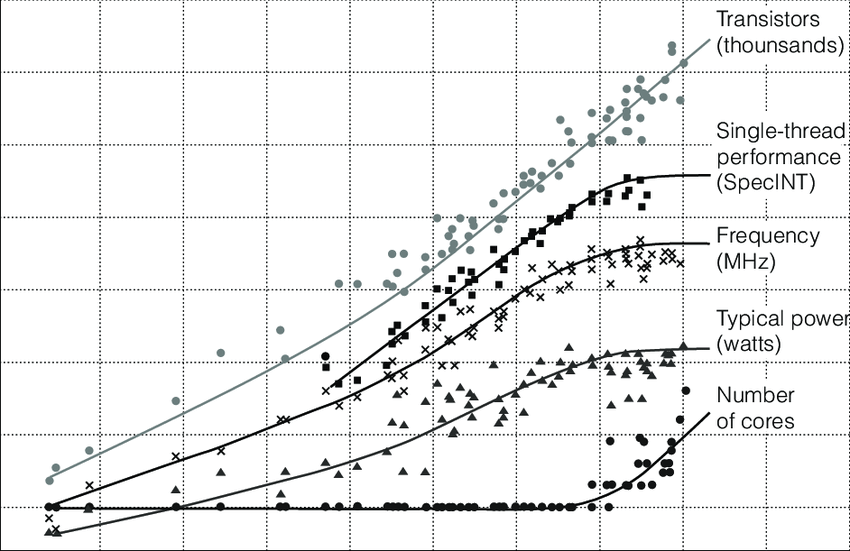
\includegraphics[width=0.75\textwidth]{images/2_background/Scaling-trends-for-the-transistor-count-clock-frequency-number-of-cores-and.png}
    \caption{A diagram showing scaling trends for the transistor count, clock frequency, number of cores, and single-thread performance of microprocessor chips. Figure created by C. Batten \cite{hardwareTrendsArticle}.}
    \label{fig:scaling-trends-transistor-clock}
\end{figure}

As a result of this, the 2013 Mantevo paper notes ``future performance gains come almost solely from running sets of instructions concurrently''. There are some mechanisms which allow this to be implemented transparently to the programmer in hardware, with superscalar processing through instruction-level parallelism. However, the most performant 

Since these hardware improvements are not transparent to the programmer, hardware-software co-design, defined by the Mantevo paper as ``collaborative simultaneous development of all system components'' became essential. As a result of this, new techniques were required for the effective co-design of high-performance systems.

\subsection{Mini-apps and the Mantevo Suite}
\label{ssec:mantevo} % 250 words

The Mantevo project at Sandia National Labs pioneered the concept of mini-apps as a tool for hardware-software co-design, publishing the Mantevo Suite in late 2012 as a collection of full-featured mini-apps for this purpose. It defines mini-apps as ``Small software programs [...] whose performance characteristics model full-scale applications, yet require only a fraction of the lines of code, making [them] easier to study, design, and re-write''.

The use of mini-apps makes hardware-software co-design with respect to very large complex application possible. This is because they can be used in place of the production application whose performance they model when making very early design decisions, without incurring the cost of massive complexity of the production application. Traditionally, mini-apps have been used to predict the performance of production applications on new hardware. However, this concept can be inverted to instead use mini-apps to predict the performance on the underlying software stack, for example the programming language of implementation.

% TODO: Consider adding more


\subsection{HPCCG}
\label{ssec:hpccg} % 500 words

% What is HPCCG

\subsubsection{Why HPCCG?}
\label{sssec:why-hpccg}
% Why was HPCCG selected

\subsubsection{Understanding HPCCG}
\label{sssec:understanding-hpccg}
% Understanding HPCCG


\subsection{Performance, Productivity, and Portability}
\label{ssec:p3hpc} % 500 words

% How the concept of mini-apps tie into general principles of pragmatic HPC engineering


\subsection{HPC software}
\label{ssec:hpc-tools} % 250 words


\subsubsection{HPC packages}
\label{sssec:hpc-packages}
% MPI/OpenMP/Rayon/Kokkos

\subsubsection{HPC tooling}
\label{sssec:hpc-tooling}
% Existing HPC tools, like slurm/likwid I guess?
% Identify/foreshadow niches which will be filled later



\section{Literature review} % 750 words
\label{sec:literature-review}

% Despite Rust being a relatively young language, its popularity has lead to academic investigations of its suitability for many tasks.
Rust's popularity has lead to academic investigations of its suitability for many tasks, despite it being a relatively young language. This literature review will start with a paper discussing the overall landscape of language performance for High-Performance Computing, comparing a single workload across 10 languages. Then, it will critically evaluate a number of performance analyses of Rust in High-Performance Computing, in order to cover a variety of techniques, from serial to highly parallel, and a variety of benchmark types, from algorithm snippets to full codebases. This project differs from existing work, as no existing analysis covers the implementation of an established mini-application to highly-parallel clustered compute, and it will include an assessment of practical suitability beyond just performance measurements. Furthermore, it will go beyond comparison to build tooling and workflows to directly improve any issues identified during this assessment.

% Benchmarking the Parallel 1D Heat Equation Solver in Chapel, Charm++, C++, HPX, Go, Julia, Python, Rust, Swift, and Java
Diehl et al. present a general overview of the landscape of language performance for a representative High-Performance Computing workload in their paper ``Benchmarking the Parallel 1D Heat Equation Solver in Chapel, Charm++, C++, HPX, Go, Julia, Python, Rust, Swift, and Java'' \cite{diehlBenchmarkingParallel1D2023}. This paper selects a 1D heat diffusion solver algorithm to implement as it uses block-structured meshes, which are commonly used in high-performance computing applications. It then goes on to qualititavely discuss the experience of implemeting the algorithm in the different languages, and suggests a quantitative metric for assesing implementation difficulty using a Constructive Cost Model (COCOMO) \cite{}. Finally, it benchmarks these implementations across three different hardware architectures, and constructs a plot comparing program runtime against its metric for implementation difficulty, duplicated in Figure \ref{fig:1d_heat_results}. The paper concludes that ``one solution does not fit all'', but names C++ as a common choice as it is both popular and performant, whilst noting Rust's ``innovative ideas will make it ideally suited for many applications''.

\begin{figure}[H]
    \centering
    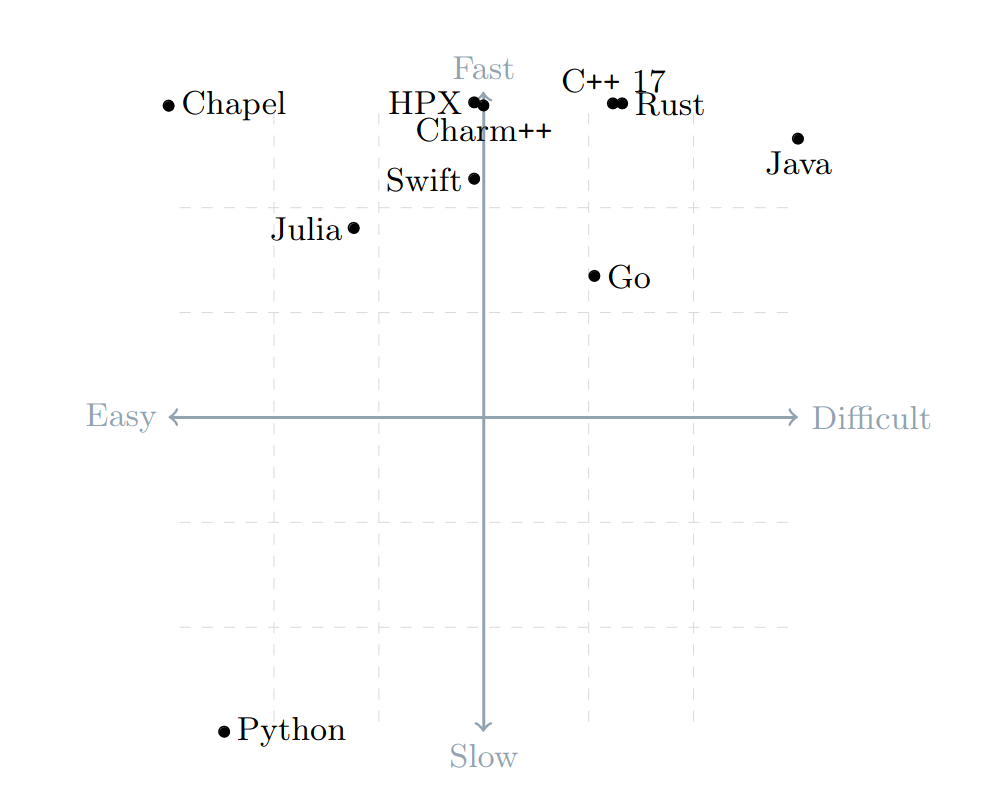
\includegraphics[width=0.75\textwidth]{images/2_background/1d_heat_results.png}
    \caption{A summary plot from Diehl et al.'s paper \cite{diehlBenchmarkingParallel1D2023}, showing ``two-dimensional classification using the computational time and the COCOMO model''.}
    \label{fig:1d_heat_results}
    % TODO: Check paper website for permission to reproduce
\end{figure}

Diehl et al. provide a strong empirically-backed analysis of the landscape of languages in the context of High-Performance Computing, and provide source code as a GitHub repository \cite{} along with naming the multiple processors used for benchmarking, allowing reproducibility of their results. However, they explicitly do not provide their measurements other then in plots, choosing ``not to name a winner with respect to speed''. Additionally, they do not provide details on their test methodology beyond naming the metrics measured and the names of hardware they used. Providing concrete results, along with a more specific methodology such as thread counts, memory size, or number or experiment re-runs would provide much more confidence in the conclusions drawn. % Note about tools to do this?
Finally, their future work notes that the selected algorithm only runs on a single CPU, and as such does not explore using MPI for distributing compute over a clustered resource, nor does it explore GPU support using a language like CUDA, nor abstractions layers like Kokkos.

% Rust language for supercomputing applications
% Serial, parallel, and MPI - but on non-standard small code snippet benchmarks. Present but flawed methodology.
Bychkov and Nikolskiy examine the readiness of the Rust language for supercomputer applications in their paper ``Rust Language for Supercomputing Applications'' \cite{bychkovRustLanguageSupercomputing2021}. The main contribution of this paper is the critical comparison of Rust and C++ over a set of benchmarks. The first benchmark characterises serial performance via a handwritten implementation of the matrix multiplication algorithm in each language. The authors note that na\"ive rust implementations perform poorly in comparison with C++, but writing Rust in an idiomatic way and leverage optimisation techniques can close this performance gap. A later benchmark characterises the performance of shared-memory parallelism via multi-threading, using OpenMP and Rayon for C++ and Rust respectively, finding that both have similar performance and scaling characteristics on the selected benchmark. The final benchmark compares the C++ native implementation of the MPI specification with the Rust bindings to it. The paper notes that the since the Rust bindings are \mintinline{rust}{safe} and leverage the rich type system, they provide many desirable properties such as guarantees of memory and thread safety and minimising boilerplate. The paper concludes that Rust is competitive to C++ for the benchmarks it explored, and that sufficient tooling exists for writing parallel code.

Bychkov and Nikolskiy present an empirically-backed analysis directly comparing Rust and C++ only across a number of different benchmarks, contrasting Diehl et al. by providing a more specific analysis rather than a general view of the landscape. The paper gives good reproducibility by clearly stating the benchmarking methodology, including machine specifications, operating system, and compiler versions. However, the choice of methodology for non-clustered machines has weaknesses. Notably, the benchmarks were run on a laptop, which can introduce noise into performance measurements if other applications are running in the background. Furthermore, the benchmarks are run under Windows Subsystem for Linux, a virtualisation technology, which significantly impacts program performance and may not be comparable to benchmarks run on unvirtualised systems. Finally, although the MPI benchmarks are run on a compute cluster which avoids the previously itemised issues, the results appear erroneous, with the authors noting ``we discovered [an] unexpected difference between Rust and C++ performance in MPI latency benchmarks'', and stating intent to re-validate the results.


% Performance vs Programming Effort between Rust and C on Multicore Architectures: Case Study in N-Body
% https://github.com/ManuelCostanzo/Gravitational_N_Bodies_Rust (250 lines of rust)
Costanza et al. investigate the difference between both performance and programming effort between Rust and C for N-body simulations in their paper ``Performance vs Programming Effort between Rust and C on Multicore Architectures: Case Study in N-Body'' \cite{costanzoPerformanceVsProgramming2021}. The paper introduces Rust as a programming language which may be suitable for High-Performance Computing due to its ownership model avoiding the need for garbage collection, and its strong support for shared-memory parallelism. It then discusses the implementation and performance optimisation of C and Rust to the gravitational n-body problem, a simple and well-known computational task. It finally compares the both the performance and programming effort of the C and Rust implementations. The paper concludes that Rust is either equally performant or slightly ($1.18\times$) slower depending on the data type precision, but that this may change with future compiler updates, and Rust requires a lower programming both in terms of lines of code and ease of parallelisation.

Costanza et al. provide a very compelling empirically-backed analysis comparing Rust and C++, which differs from Bychkov and Nikolskiy by considering both the practical implications of programming effort, and making the comparison on a representative code sample rather than simple benchmarks. However, the paper does not consider highly-parallel clustered compute using technologies such as MPI. The paper provides a discussion of practical techniques for writing performant Rust beyond threading, including use of SIMD intrinsics and custom memory allocators, along with a compelling and unbiased performance analysis of Rust and C++.

% Emerging technologies, Rust in HPC
% Parallel only implementation for non-standard very small full application for C++ and Fortran, good methodology. Poor Rust implementation
% https://github.com/lmoran94/eurocc_cfd (112 lines of Rust)
Moran and Bull investigate the performance of Rust as compared with C++ and FORTRAN on computational fluid dynamics problems in their technical report ``Emerging Technologies: Rust in HPC'' \cite{moranEmergingTechnologiesRust2023}. This paper is similar to Costanza et al. in comparing a small custom codebase which is representative of High-Performance Computing workloads, but differs by including FORTRAN in its comparisons, along with placing a greater focus on performance analysis and scaling, and less consideration to programming effort. The paper 

% Criticism

% Towards Safe HPC: Productivity and Performance via Rust Interfaces for a Distributed C++ Actors Library
Parrish et al. present a framework for writing parellel programs, including a performance analysis of this framework, in their paper ``Towards Safe HPC: Productivity and Performance via Rust Interfaces for a Distributed C++ Actors Library (Work in Progress) [sic]'' \cite{parrishSafeHPCProductivity2023}. The paper concludes that their ``Rust versions of the original application performed on par with the respective C++ verions''. To support this claim, the paper includes figures showing the performance of Rust and C++ for various kernels, such as the one shown replicated in Figure \ref{actors_bad_histogram}.

\begin{figure}[H]
    \centering
    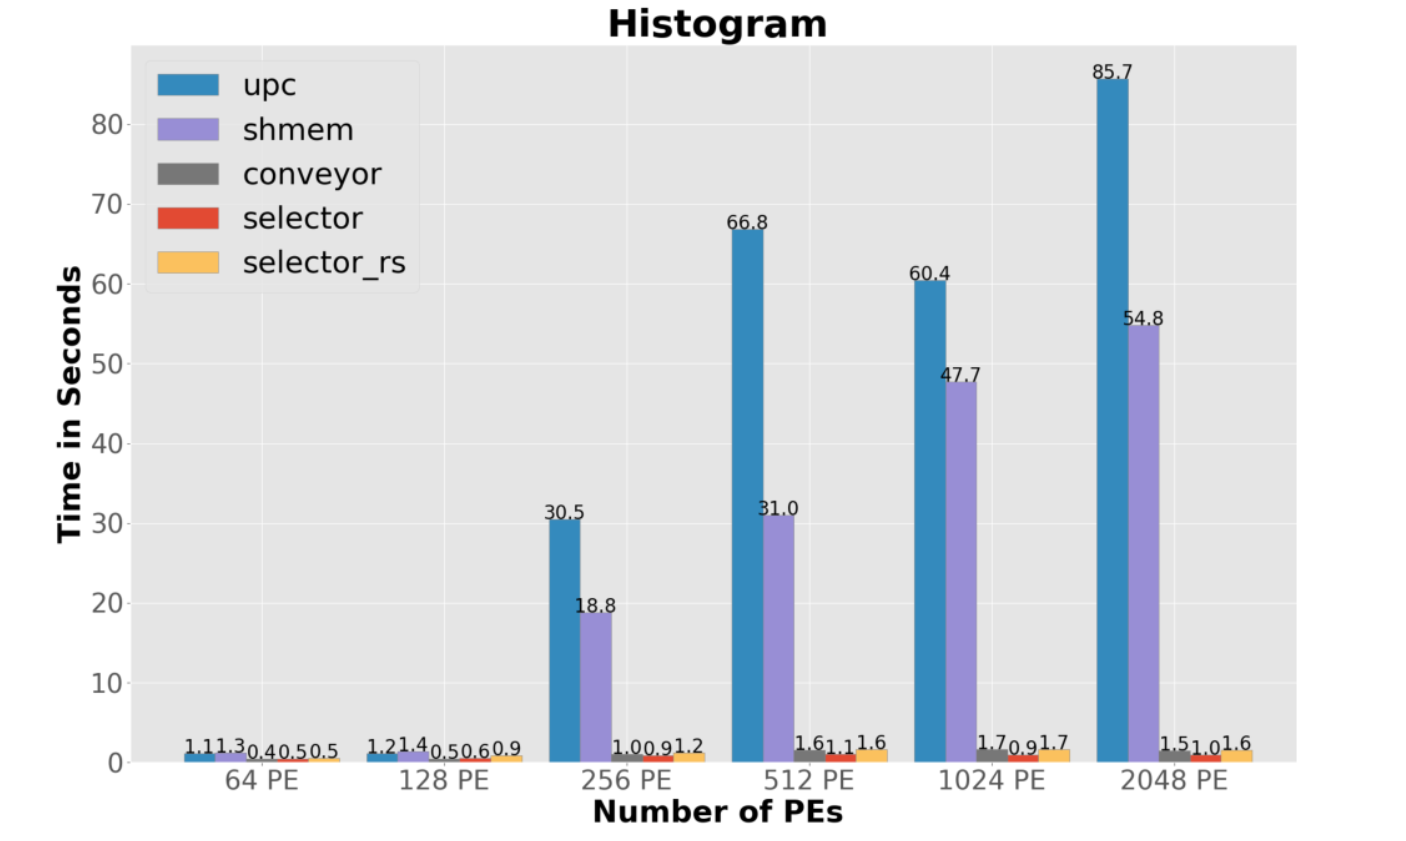
\includegraphics[width=0.75\textwidth]{images/2_background/actors_bad_histogram.png}
    \caption{A figure showing the performance of the Histogram kernel across various implementations, from Appendix A of Parrish et al. \cite{parrishSafeHPCProductivity2023}.}
    \label{fig:actors_bad_histogram}
    % TODO: Check paper website for permission to reproduce
\end{figure}

However, the data shown in Figure \ref{actors_bad_histogram} does not support the claim that Rust is as performant as C++. The inclusion of the much slower ``upc'' and ``shmem'' implementations skew the scale of the plot so Rust and C++ versions look the same, but in fact by examining the data labels we can see the implementation is on average $1.46\times$ slower for this kernel, which is non-negligibly slower. This aligns with the results of other publications such as Costanza et al. who observed a $1.18\times$ slowdown, and noted it as such. In the authors opinion, this paper is emblematic of common problem in literature about the Rust programming language -- the bias held by some that the Rust programming language is better in all respects than other programming languages. Despite the fact that the data in the paper shows that the Rust implementation is slower \ref{actors_bad_histogram}, the data is presented in a disingenuous way in order to draw the conclusion that it is equally performant.


% Rust programming language in the high-performance computing environment
% Rayon + MPI implementation of code snippet, run data but no source code


%% Summary
In summary, there is existing research around the suitability of Rust in High-Performance Computing, which broadly concludes that Rust is slightly slower than C++, but provides other benefits which might mitigate this fact. The existence of publications in this area is compelling that it is a relevant and difficult question to answer. However, there is still space for novel contribution in this area, for example by assessing highly-parallel clustered compute as applied to a standard mini-application, rather than a simple benchmark or toy example. Furthermore, many existing papers do not focus on reproducibility of results, by ommiting the source code, research methodology, or recorded results. Finally, none of the papers provide tooling to assist in the process of translating High-Performance Computing codebases, giving a further opportunity for novel contribution.